\chapter{從粒子力學到經典場論}

\section{什麼是場}

上一講從不變作用量出發，建立了相對論性粒子力學。現在我們要改變動力學對象，討論的是經典場論，而非量子場論。量子力學偶爾可作為有用的對照，但本章的方程描述的是一般的經典場。電磁學是我們熟悉的背景模型：電磁波在空間中傳播，並與帶電粒子相互作用。我們先從更簡單的場開始。

時空可以有許多空間座標，但只有一個時間座標。寫成
\begin{equation}
x^\mu=(t,x^1,\ldots,x^d),
\end{equation}
其中空間指標為 \(i=1,\ldots,d\)。數 \(d\) 可以是三，如同我們的世界；也可以是一、二、九、二十五，或模型所需的任何其他數值。此處重要的不對稱之處，是時間方向仍然只有一個。本講不試圖解釋為何具有多個時間方向的理論如此困難；它只是採用一般因果物理所使用的單一時間架構。

場是一種可測量的量，其值可能隨位置和時間而變化。溫度就是一個簡單的例子：
\begin{equation}
T=T(\mathbf{x},t).
\end{equation}
它為每個事件指定一個數值，因此是標量場。風的速度也會隨空間和時間而變化，但它有大小和方向，因而具有多個分量；所以它是向量場。在相對論物理中，自然的向量有四個分量，而非三個。

本講大部分內容所討論的場只有一個分量，並以對應於 \(f\) 的希臘字母表示：
\begin{equation}
\phi=\phi(\mathbf{x},t).
\label{eq:sr4-field-definition}
\end{equation}
之後稱 \(\phi\) 為標量，意義將不止於它只有一個分量；這還表示所有慣性觀察者在同一個物理事件處，對 \(\phi\) 所指定的值都相同。建立變分力學之後，才會引入這個變換律。

\section{粒子模型}

\subsection{稱為 \texorpdfstring{\(\phi\)}{phi} 的座標}

要進入場論，最快的方法是先退回到一般的非相對論性粒子。設粒子沿直線運動，但把它的座標稱為 \(\phi\)，而不是 \(x\)。座標沒有非得命名為 \(x\) 的數學理由；選用這個不尋常的名稱，是為了讓接下來的類比一目了然。把時間畫成水平軸，粒子的整段歷史便是一條曲線 \(\phi(t)\)，可以經過正值，也可以經過負值。

固定初始時刻 \(a\) 和終止時刻 \(b\) 時，作用量為
\begin{align}
A[\phi]
&=\int_a^b dt\,L(\phi,\dot\phi),\\
L(\phi,\dot\phi)
&=\frac{m}{2}\dot\phi^{\,2}-V(\phi).
\label{eq:sr4-particle-lagrangian}
\end{align}
尤拉--拉格朗日方程為
\begin{equation}
\frac{d}{dt}\left(\frac{\partial L}{\partial\dot\phi}\right)
-\frac{\partial L}{\partial\phi}=0.
\label{eq:sr4-particle-el}
\end{equation}
對於 \eqref{eq:sr4-particle-lagrangian} 中的拉格朗日量，
\begin{equation}
\frac{\partial L}{\partial\dot\phi}=m\dot\phi,
\qquad
\frac{\partial L}{\partial\phi}=-\frac{dV}{d\phi},
\end{equation}
因此
\begin{equation}
\boxed{m\ddot\phi=-\frac{dV}{d\phi}}.
\label{eq:sr4-newton}
\end{equation}
這就是以 \(\phi\) 為座標寫出的牛頓方程。

\begin{figure}[htbp]
\centering
\includegraphics[width=0.90\textwidth]{lecture_04_figure_01.png}
\caption{一般的尤拉--拉格朗日方程，以及座標 \(\phi(t)\) 對應的牛頓方程。}
\lectureframe{00:10:18}
\end{figure}

端點固定時，物理路徑使作用量取駐值。本講常說 \emph{極小}，但精確來說，作用量取的是駐值：路徑可能使它取極小值、極大值，或其他駐值。一個有用的想像方式，是把時間區間分成許多小段。如此一來，作用量就成為 \(\phi\) 在各個取樣點取值的函數。保持端點不動，改變這些取樣值，並分別對每個值求導；這正是尤拉--拉格朗日方程的有限維前身。

\subsection{作為 \texorpdfstring{\(0+1\)}{0+1} 維理論的力學}

現在想像一個有時間、沒有空間維度的世界。它的空間只有一個點。那裡的場無法依賴位置，因為沒有位置可供依賴；它只能是函數 \(\phi(t)\)。因此，一個座標的普通粒子力學，也可以看成 \(0+1\) 維中的場論。數學並沒有改變，只是詮釋從粒子的位置改成了無空間世界中的場值。

\begin{figure}[htbp]
\centering
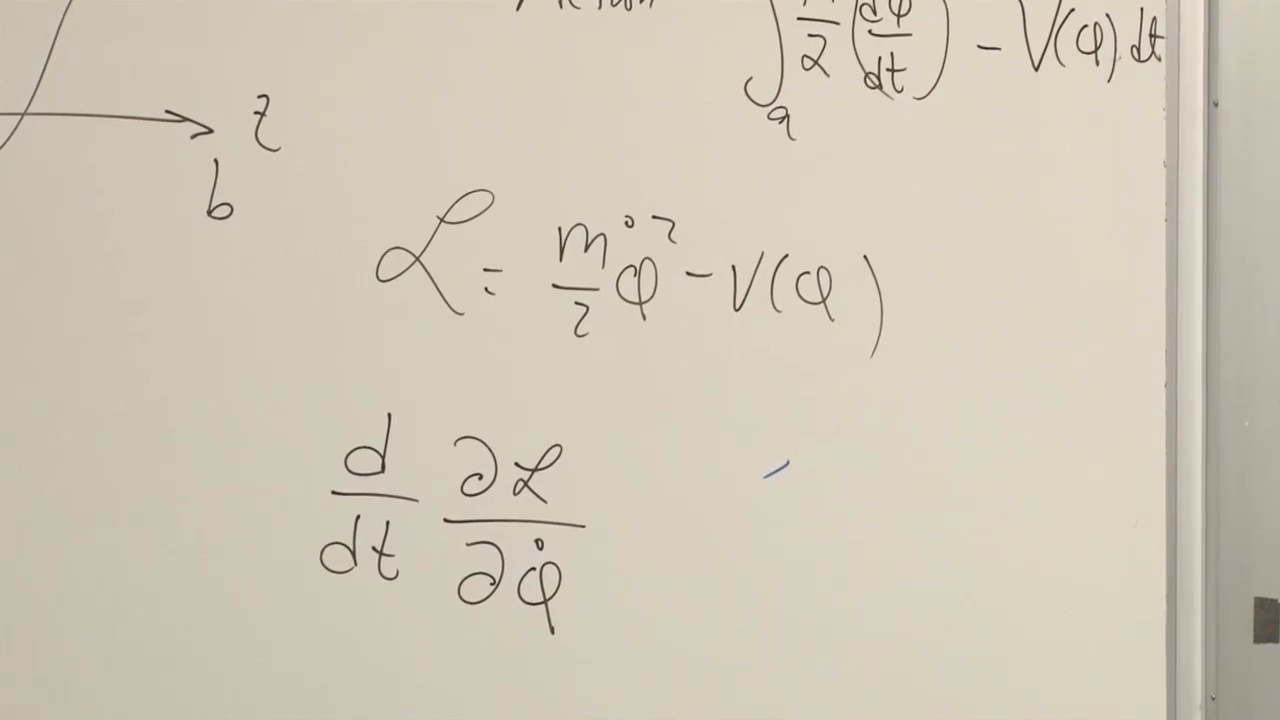
\includegraphics[width=0.90\textwidth]{lecture_04_figure_02.png}
\caption{取樣後的歷史 \(\phi(t)\)：粒子軌跡，換個詮釋後則是 \(0+1\) 維中的場歷史。}
\lectureframe{00:14:30}
\end{figure}

\begin{classroomqa}
\audiencequestion{沒有空間維度時，勢能會消失嗎？}
\lecturerresponse{不會。消失的是空間變化，場仍有一個值。能量仍可能透過 \(V(\phi)\) 依賴這個值。以粒子的觀點來看，上下移動曲線會改變勢能；以場的觀點來看，\(\phi\) 的不同取值各自對應不同的勢能。\lecturetimestamp{00:15:00}}
\end{classroomqa}

\begin{classroomqa}
\audiencequestion{除了想像完全沒有空間，也可以想像一般空間中的場只依賴時間嗎？}
\lecturerresponse{可以。就此而言，兩者的局部數學形式相同：所有空間導數都為零，只剩下 \(\phi(t)\)。稱這種情形為 \(0+1\) 維理論，是為了單獨考察這個約化後的結構；較大世界中的空間均勻場，也能提供相同的直觀理解。\lecturetimestamp{00:16:25}}
\end{classroomqa}

現在可以看出這段迂迴的用意：我們已知適用於只依賴一個座標，也就是時間的場之作用量原理。接著可以依循這個形式，推想適用於依賴所有時空座標之場的作用量原理。

\section{時空上的場歷史}

\subsection{從曲線到曲面}

在 \(1+1\) 維時空中，時空本身是一個以 \(t\) 和 \(x\) 為座標的平面。場值 \(\phi(x,t)\) 則提供第三個方向。因此，場的歷史不是曲線，而是時空平面上方的一個曲面。這個曲面可以高於或低於零，因為標量場不必是正值。

\begin{figure}[htbp]
\centering
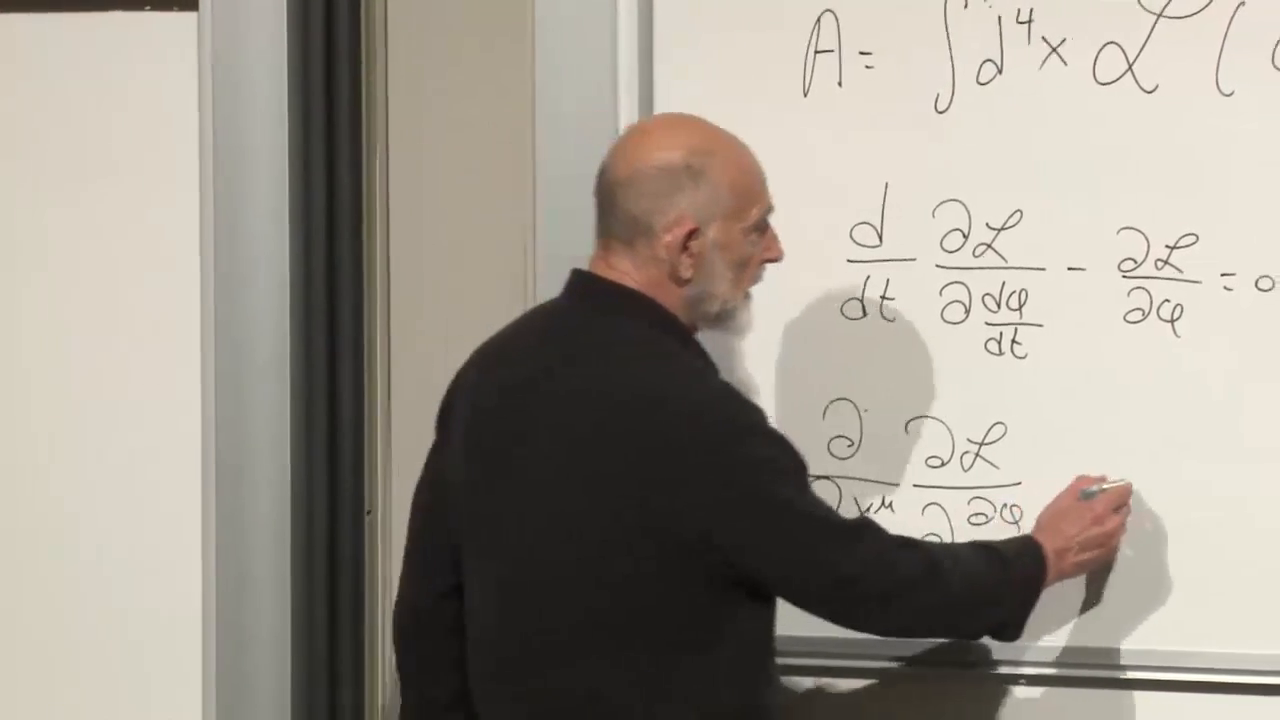
\includegraphics[width=0.90\textwidth]{lecture_04_figure_03.png}
\caption{畫成曲面的標量場歷史，位於 \(1+1\) 維時空平面上方。}
\lectureframe{00:20:46}
\end{figure}

我們的物理時空稱為 \(3+1\) 維，包含三個空間維度和一個時間維度。桌面模型是 \(2+1\) 維的，而受限於一條線上的珠子則可用來想像 \(1+1\) 維世界。要繪出 \(\phi\)，還需要額外一個軸，因此即使是 \(3+1\) 維的情形，也無法忠實地畫出來；但定義十分明確：完整的歷史會為每個時空事件指定一個 \(\phi\) 值。

\subsection{從固定端點到固定邊界資料}

粒子的變分問題固定兩個端點，並改變兩端之間的曲線。場論中的對應做法，是選定一個時空區域，固定該區域邊界上的 \(\phi\)，並改變內部的 \(\phi\)。這個區域可以是 \(1+1\) 維圖中的矩形，也可以是高維時空中的任何適當區域。

\begin{figure}[htbp]
\centering
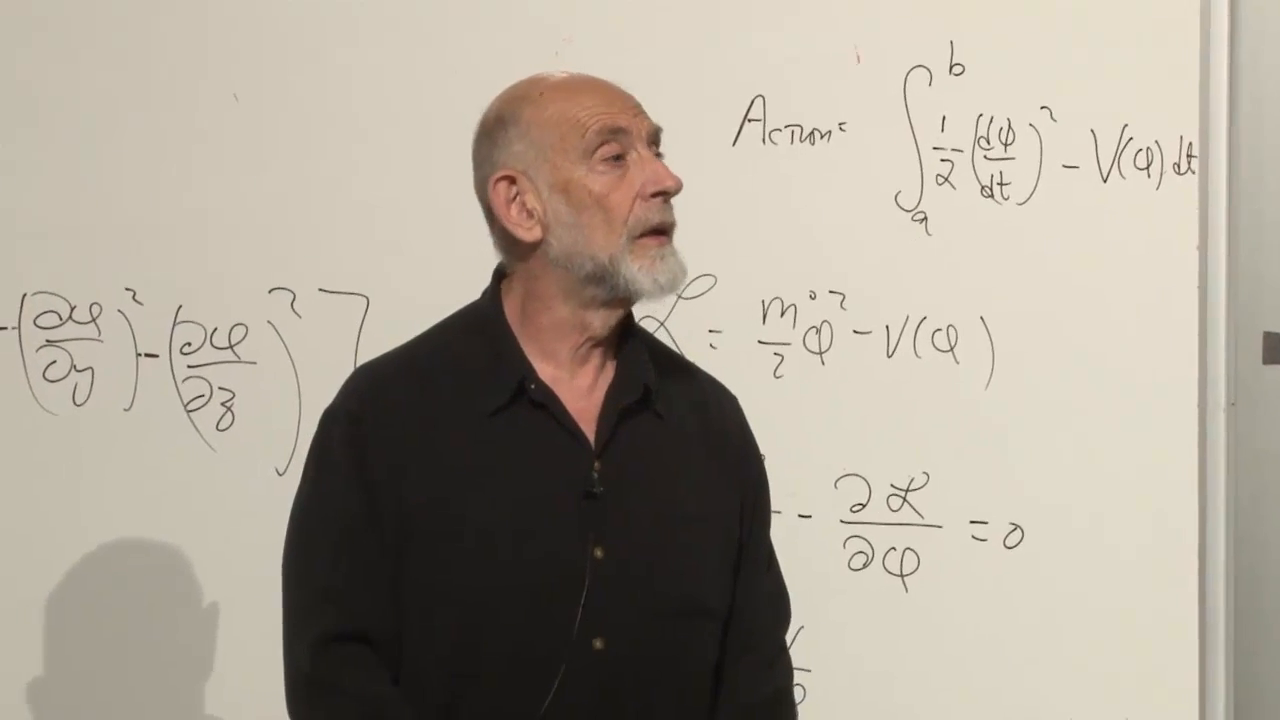
\includegraphics[width=0.90\textwidth]{lecture_04_figure_04.png}
\caption{固定時空區域的整個邊界，並改變區域內部的場。}
\lectureframe{00:24:52}
\end{figure}

\begin{classroomqa}
\audiencequestion{勢能若顯式依賴時間，拉格朗日表述還適用嗎？}
\lecturerresponse{適用。尤拉--拉格朗日表述和哈密頓表述仍然成立。一般來說，失去的是能量守恆：顯式的時間依賴會破壞時間平移對稱性。場論中的對應情形也允許顯式的時空依賴，不過這會影響相關的守恆定律。\lecturetimestamp{00:23:49}}
\end{classroomqa}

\begin{classroomqa}
\audiencequestion{對矩形場區域而言，固定的是頂邊和底邊，還是整個邊界？}
\lecturerresponse{在這個變分構造中，固定的是整個邊界，也就是 \(1+1\) 維矩形的四條邊。場只在內部改變。這直接對應於粒子力學中固定兩個端點的做法。\lecturetimestamp{00:24:24}}
\end{classroomqa}

固定整個邊界，指的是推導方程時所採用的變分條件。若將推導出的雙曲型場方程視為物理演化問題，較常見的做法是指定適當的初始資料，讓方程向前演化。

\section{作用量與場的尤拉--拉格朗日方程}

\subsection{拉格朗日密度}

把時空區域劃分為小胞元，並假設作用量是各胞元局部貢獻的總和。在連續極限下，這個總和便成為時空積分：
\begin{equation}
A[\phi]
=
\int_{\Omega} d^4x\,
\mathcal{L}\!\left(
\phi,\partial_\mu\phi;x^\mu
\right),
\qquad
d^4x=dt\,dx\,dy\,dz.
\label{eq:sr4-field-action}
\end{equation}
量 \(\mathcal{L}\) 稱為拉格朗日密度。\(\mathcal{L}(\phi,\partial_\mu\phi;x^\mu)\) 中的分號用來區分動力學變數與可能存在的顯式座標依賴。在均勻的封閉系統中，通常沒有後者，但變分形式並未禁止它。

緊湊的記號
\begin{equation}
\partial_\mu\phi
\equiv
\frac{\partial\phi}{\partial x^\mu}
\end{equation}
將時間導數和空間導數統一表示。也可以使用本講的分量記號，寫成
\begin{equation}
\begin{aligned}
\phi_t&=\frac{\partial\phi}{\partial t},\\
\phi_x&=\frac{\partial\phi}{\partial x},\\
\phi_y&=\frac{\partial\phi}{\partial y},\\
\phi_z&=\frac{\partial\phi}{\partial z}.
\end{aligned}
\label{eq:sr4-component-derivatives}
\end{equation}
場可以有多個，就像粒子可以有多個座標一樣。目前只有一個場 \(\phi\)。

符號 \(d^4x\) 只是四維座標測度的簡寫。若時空維度不同，就要改用 \(d^Dx\)。在 \(0+1\) 維的原型中，\(D=1\)，而 \(d^1x\) 就只是 \(dt\)。

\begin{figure}[htbp]
\centering
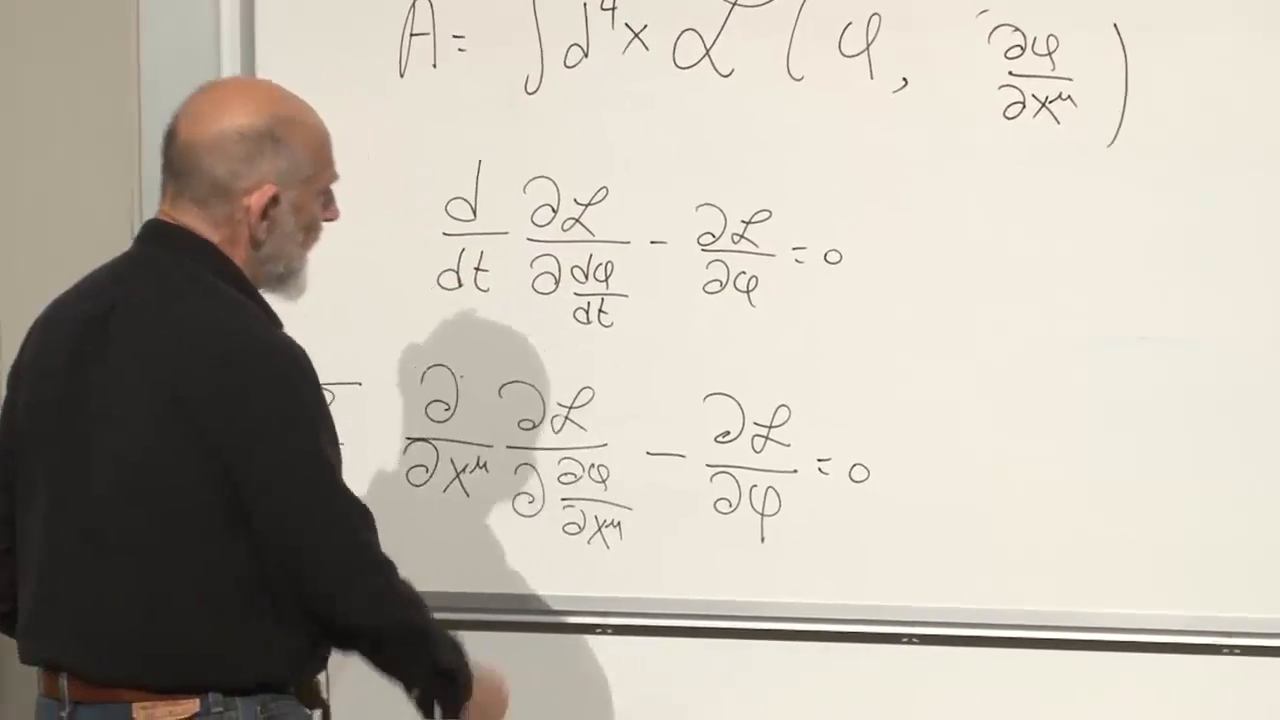
\includegraphics[width=0.90\textwidth]{lecture_04_figure_05.png}
\caption{作用量密度寫成 \(\phi\) 及其時空導數的局部函數。}
\lectureframe{00:32:51}
\end{figure}

\begin{classroomqa}
\audiencequestion{拉格朗日密度也可以依賴 \(x,y,z\) 本身嗎？}
\lecturerresponse{可以，就像粒子的拉格朗日量可以顯式依賴 \(t\) 一樣。對平移不變的封閉系統而言，通常不會有這種依賴；但顯式的座標依賴並不會使這套形式失效。\lecturetimestamp{00:30:29}}
\end{classroomqa}

\begin{classroomqa}
\audiencequestion{目前的構造只適用於標量場，還是具有一般性？}
\lecturerresponse{目前的變分形式具有一般性。只寫一個分量，表示這裡以標量場為例。向量場或一組場會有額外的分量標記，因此必須對每個分量分別作變分。\lecturetimestamp{00:31:00}}
\end{classroomqa}

\subsection{格點圖像}

在細密的時空格點上，導數會變成相鄰場值之間的有限差分。於是作用量就成為多個變數的普通函數。若一個方向有十個點，另一個方向有八個點，格網便已有八十個場變數。細化格網會增加變數的數目，但極小化的規則仍很簡單：對每個內部格點的場值求作用量的導數，並令結果為零。

\begin{figure}[htbp]
\centering
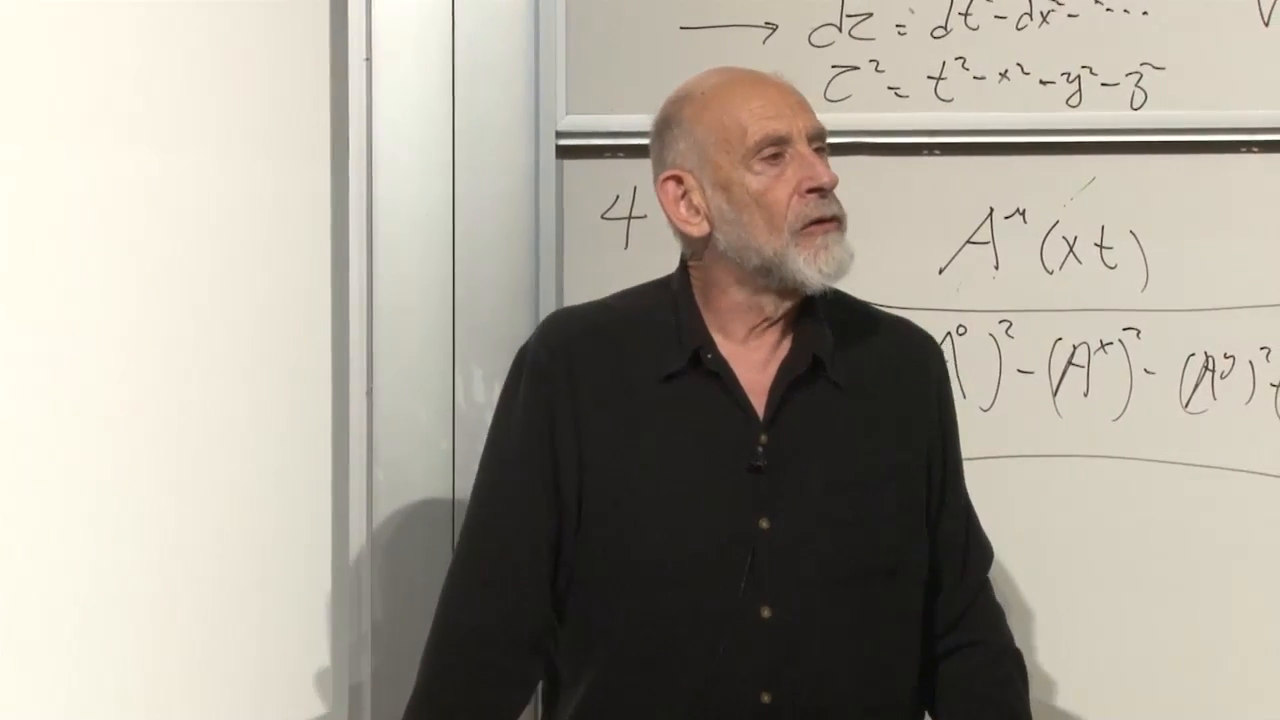
\includegraphics[width=0.90\textwidth]{lecture_04_figure_06.png}
\caption{將時空區域劃分成胞元；在取連續極限之前，作用量因此是多變數的普通函數。}
\lectureframe{00:34:05}
\end{figure}

取連續極限後，便得到場的尤拉--拉格朗日方程：
\begin{equation}
\boxed{
\partial_\mu
\left[
\frac{\partial\mathcal{L}}
{\partial(\partial_\mu\phi)}
\right]
-
\frac{\partial\mathcal{L}}{\partial\phi}
=0
}.
\label{eq:sr4-field-el}
\end{equation}
重複出現的 \(\mu\) 表示對所有時空方向求和。若不用求和簡記，同一方程可寫成
\begin{align}
&
\frac{\partial}{\partial t}
\left(\frac{\partial\mathcal{L}}{\partial\phi_t}\right)
+
\frac{\partial}{\partial x}
\left(\frac{\partial\mathcal{L}}{\partial\phi_x}\right)
+
\frac{\partial}{\partial y}
\left(\frac{\partial\mathcal{L}}{\partial\phi_y}\right)
\nonumber\\
&\hspace{3em}
+
\frac{\partial}{\partial z}
\left(\frac{\partial\mathcal{L}}{\partial\phi_z}\right)
-
\frac{\partial\mathcal{L}}{\partial\phi}
=0.
\label{eq:sr4-field-el-expanded}
\end{align}
第一項是熟悉的粒子力學項。場論則在每個空間方向都多出一個類似的項。最後一項 \(-\partial\mathcal{L}/\partial\phi\) 則保持不變。

\begin{figure}[htbp]
\centering
\includegraphics[width=0.90\textwidth]{lecture_04_figure_07.png}
\caption{上下並列呈現的一維尤拉--拉格朗日方程及其時空推廣。}
\lectureframe{00:38:44}
\end{figure}

這個領域也稱為連續介質力學。依自由度而定，同一套數學可以描述流體流動、彈性位移，或其他連續介質。

\begin{classroomqa}
\audiencequestion{同樣的方程也適用於有空間、沒有時間的世界嗎？}
\lecturerresponse{適用，可將它視為純空間的變分問題。物理上，尋找靜態解時正是這麼做：假設場不隨時間變化，去掉所有時間導數，再求解剩下的空間方程。靜態的電場或磁場位形就是一個例子。\lecturetimestamp{00:40:05}}
\end{classroomqa}

\section{猜想最簡單的標量場動力學}

\subsection{為何符號不能全都相同}

回到粒子的動能項 \(\tfrac12\dot\phi^2\)，把無關緊要的整體係數設為一，並嘗試將它推廣。第一個猜想可能是
\begin{equation}
\mathcal{L}_{+}
=
\frac12
\left[
\phi_t^2+\phi_x^2+\phi_y^2+\phi_z^2
\right].
\label{eq:sr4-all-plus}
\end{equation}
這是一個有用的錯誤嘗試，因為它以相同的符號對待時間和空間。由此得到的方程不會呈現波傳播所需的雙曲結構。正確的相對論性組合對時間採用一種符號，對空間則採用相反的符號。

\begin{classroomqa}
\audiencequestion{全正號的表示式之所以不對，是因為拉格朗日量應具有相對論不變性嗎？}
\lecturerresponse{這是更深一層的答案，而且是正確的。講座先從較直觀的角度得到符號安排：波在時間中的演化有別於在空間中的變化，因此時間不能完全像另一個空間座標那樣進入表示式。接著，洛倫茲不變性會將這個直覺化為精確規則。\lecturetimestamp{00:43:19}}
\end{classroomqa}

恢復特徵速度 \(c\) 後，簡單的標量拉格朗日密度為
\begin{equation}
\boxed{
\mathcal{L}
=
\frac12
\left[
\frac{1}{c^2}\phi_t^2
-\phi_x^2-\phi_y^2-\phi_z^2
\right]
-V(\phi)
}.
\label{eq:sr4-scalar-lagrangian}
\end{equation}
對相對論性場而言，\(c\) 是光速。在連續介質模型中，它也可以是聲速、彈性波速，或其他特徵傳播速度。

整體因子 \(1/2\) 是一種約定，就像 \(\tfrac12m\dot\phi^2\) 中的情形一樣。把整個作用量乘上非零常數，不會改變其駐定路徑；這種約定決定了方程中參數的命名和正規化方式。一旦選定正規化方式，就必須始終一致地使用。

\begin{classroomqa}
\audiencequestion{空間梯度項能否視為勢能的一部分？}
\lecturerresponse{可以。若將拉格朗日量整理成動能減勢能的形式，動能部分包含時間導數；不含時間導數的項，包括空間梯度項和 \(V(\phi)\)，都歸在勢能一側。在相對論理論中，這些項的相對符號最終來自洛倫茲度規。\lecturetimestamp{00:45:37}}
\end{classroomqa}

\subsection{波動方程}

將 \eqref{eq:sr4-field-el} 代入。導數項為
\begin{equation}
\frac{\partial\mathcal{L}}{\partial\phi_t}
=\frac{1}{c^2}\phi_t,
\qquad
\frac{\partial\mathcal{L}}{\partial\phi_i}
=-\phi_i,
\end{equation}
而
\begin{equation}
\frac{\partial\mathcal{L}}{\partial\phi}
=-\frac{dV}{d\phi}.
\end{equation}
因此
\begin{equation}
\begin{aligned}
&\boxed{
\frac{1}{c^2}\frac{\partial^2\phi}{\partial t^2}
-\nabla^2\phi
+\frac{dV}{d\phi}
=0
},\\[0.5em]
\nabla^2
&=
\frac{\partial^2}{\partial x^2}
+\frac{\partial^2}{\partial y^2}\\
&\quad
+\frac{\partial^2}{\partial z^2}.
\end{aligned}
\label{eq:sr4-general-scalar-eom}
\end{equation}

若 \(V=0\)，此式便化為
\begin{equation}
\boxed{
\frac{1}{c^2}\phi_{tt}-\nabla^2\phi=0
},
\label{eq:sr4-wave-equation}
\end{equation}
也就是波動方程。講座認出這個方程，但暫不求解。它的解會以速度 \(c\) 傳播擾動。

\begin{figure}[htbp]
\centering
\includegraphics[width=0.90\textwidth]{lecture_04_figure_08.png}
\caption{辨認為波動方程的一維形式 \(c^{-2}\phi_{tt}-\phi_{xx}=0\)。}
\lectureframe{00:50:30}
\end{figure}

\subsection{耦合諧振子的場}

現在選取二次勢：
\begin{equation}
V(\phi)=\frac12\mu^2\phi^2,
\qquad
\frac{dV}{d\phi}=\mu^2\phi.
\label{eq:sr4-quadratic-potential}
\end{equation}
若 \(\phi\) 代表粒子的位置，這就是彈簧常數為 \(\mu^2\) 的諧振子勢能。對場而言，
\begin{equation}
\boxed{
\frac{1}{c^2}\phi_{tt}-\nabla^2\phi+\mu^2\phi=0
}.
\label{eq:sr4-klein-gordon}
\end{equation}
若沒有空間導數，這個方程就只是「加速度加上常數乘以位移等於零」。梯度項會耦合相鄰位置的場值，使振子構成可傳播波的連續介質。在相對論場論中，\eqref{eq:sr4-klein-gordon} 稱為有質量的克萊因--戈登方程；在經典理論中，\(\mu\) 是修正波傳播的逆長度尺度。

\begin{figure}[htbp]
\centering
\includegraphics[width=0.90\textwidth]{lecture_04_figure_09.png}
\caption{二次勢，以及包含恢復項 \(\mu^2\phi\) 的波動方程。}
\lectureframe{00:52:38}
\end{figure}

\begin{classroomqa}
\audiencequestion{為什麼運動方程中不見了 \(V=\tfrac12\mu^2\phi^2\) 裡的因子 \(1/2\)？}
\lecturerresponse{對 \(\phi^2\) 微分會產生因子二。加入慣用因子 \(1/2\)，正是為了讓 \(dV/d\phi=\mu^2\phi\)；這和 \(V(x)=\tfrac12kx^2\) 產生恢復力 \(-kx\) 的道理相同。\lecturetimestamp{00:53:17}}
\end{classroomqa}

這個方程是線性的：\(\phi\) 及其導數都只以一次方出現。若運動方程中出現 \(\phi^2\) 或 \(\phi\,\partial_\mu\phi\) 等項，動力學就會變成非線性。

\section{洛倫茲標量與四維向量}

\subsection{作用量必須與參考系無關}

單靠變分方法可以定義許多不同的場論。相對論進一步要求：作用量在每個慣性參考系中都具有相同的值和形式。自由粒子的作法，是沿著世界線積分不變的固有時間 \(d\tau\)。場的作用量則對時空積分，因此其中的局部構件必須依適當的方式變換。

在正洛倫茲變換下，時空測度保持不變：\(d^4x'=d^4x\)。因此，只要要求拉格朗日密度是洛倫茲標量即可：
\begin{equation}
\mathcal{L}'(x')=\mathcal{L}(x).
\label{eq:sr4-lagrangian-scalar}
\end{equation}

\subsection{標量場}

標量場遵守
\begin{equation}
\boxed{\phi'(x')=\phi(x)}.
\label{eq:sr4-scalar-transform}
\end{equation}
座標 \(x\) 和 \(x'\) 分別標示兩個參考系中的同一事件。觀察者使用的函數表示式可能不同，但對應到該物理事件的數值相同。

\begin{figure}[htbp]
\centering
\includegraphics[width=0.90\textwidth]{lecture_04_figure_10.png}
\caption{標量場的定義性變換律：\(\phi(x)=\phi'(x')\)。}
\lectureframe{00:59:33}
\end{figure}

溫度提供了早期的直觀例子，不過在物質介質中移動的溫度計並非完美的相對論例子。關鍵在於定義 \eqref{eq:sr4-scalar-transform}，而不是溫度計的類比。

\subsection{四維向量}

在單位制 \(c=1\) 下，沿 \(x\) 軸以速度 \(v\) 作洛倫茲推動時，變換為
\begin{equation}
\begin{aligned}
t'&=\gamma(t-vx),\\
x'&=\gamma(x-vt),\\
y'&=y,\\
z'&=z,\\
\gamma&=\frac{1}{\sqrt{1-v^2}}.
\end{aligned}
\label{eq:sr4-x-boost}
\end{equation}

\begin{figure}[htbp]
\centering
\includegraphics[width=0.90\textwidth]{lecture_04_figure_11.png}
\caption{在 \(c=1\) 單位制下，沿 \(x\) 軸作推動時的洛倫茲變換。}
\lectureframe{01:02:26}
\end{figure}

任何四個在推動下依相同方式混合的量，都構成四維向量。已經見過的例子包括 \(x^\mu\)、\(dx^\mu\)，以及四維速度 \(u^\mu=dx^\mu/d\tau\)。四維向量乘以標量後，仍是四維向量。流動的相對論性流體提供了一個場值的例子：其四維速度 \(u^\mu(x)\) 可以因事件而異。

對於與 \eqref{eq:sr4-x-boost} 相同的推動，一般四維向量滿足
\begin{equation}
\begin{aligned}
A'^0&=\gamma(A^0-vA^x),\\
A'^x&=\gamma(A^x-vA^0),\\
A'^y&=A^y,\\
A'^z&=A^z.
\end{aligned}
\label{eq:sr4-vector-boost}
\end{equation}

對一般四維向量 \(A^\mu=(A^0,A^x,A^y,A^z)\) 而言，洛倫茲範數
\begin{equation}
\boxed{
A_\mu A^\mu
=(A^0)^2-(A^x)^2-(A^y)^2-(A^z)^2
}
\label{eq:sr4-vector-norm}
\end{equation}
是標量。它的不變性與
\begin{equation}
d\tau^2=dt^2-dx^2-dy^2-dz^2
\end{equation}
的不變性，源自相同的代數理由。講座一度找不到尚未用過的字母來代表一般向量，最後接受了 \(A\)；有人建議用箭頭表示 \(A\)，這也促成了這個選擇。

\begin{figure}[htbp]
\centering
\includegraphics[width=0.90\textwidth]{lecture_04_figure_12.png}
\caption{一般四維向量場，以及用來構造不變範數的洛倫茲平方差。}
\lectureframe{01:09:06}
\end{figure}

\subsection{標量的導數}

將標量對四個時空座標分別微分，可得到四個分量：
\begin{equation}
\partial_\mu\phi
=
\left(
\frac{\partial\phi}{\partial t},
\frac{\partial\phi}{\partial x},
\frac{\partial\phi}{\partial y},
\frac{\partial\phi}{\partial z}
\right)
\qquad(c=1).
\end{equation}
嚴格來說，\(\partial_\mu\phi\) 是協向量；利用閔可夫斯基度規升高其指標後，得到 \(\partial^\mu\phi\)。在這裡的分量論證中，這項區別不影響計算，但能明確界定縮併方式：
\begin{equation}
\boxed{
\partial_\mu\phi\,\partial^\mu\phi
=
\frac{1}{c^2}\phi_t^2
-\phi_x^2-\phi_y^2-\phi_z^2
}.
\label{eq:sr4-derivative-scalar}
\end{equation}

\begin{figure}[htbp]
\centering
\includegraphics[width=0.90\textwidth]{lecture_04_figure_13.png}
\caption{由標量場的一階導數構成的不變平方差。}
\lectureframe{01:13:55}
\end{figure}

\begin{classroomqa}
\audiencequestion{這個導數的組合是拉普拉斯算子嗎？}
\lecturerresponse{不是。圖示的不變量是由一階導數構成的二次式；拉普拉斯算子則包含二階空間導數。要到作用量經變分、得到波動方程時，二階導數才會出現。\lecturetimestamp{01:13:22}}
\end{classroomqa}

\eqref{eq:sr4-scalar-lagrangian} 中的符號安排如今有了解釋，而非只是猜測。動能與梯度項的組合是洛倫茲標量 \(\partial_\mu\phi\,\partial^\mu\phi\)。因此，最簡單的二次理論為
\begin{equation}
\mathcal{L}
=
\frac12\partial_\mu\phi\,\partial^\mu\phi
-\frac12\mu^2\phi^2.
\label{eq:sr4-covariant-lagrangian}
\end{equation}

\begin{figure}[htbp]
\centering
\includegraphics[width=0.90\textwidth]{lecture_04_figure_14.png}
\caption{黑板上寫出的完整二次標量場拉格朗日量及其線性場方程。}
\lectureframe{01:19:12}
\end{figure}

\section{自由度有多少？}

知道如何構造標量之後，就可以建立許多不同的拉格朗日量。場 \(\phi\) 是標量，因此任何普通函數 \(F(\phi)\) 也都是標量，例如 \(\phi^2\)、\(\phi^3\)、\(\cosh\phi\) 等。也可以加入數值參數，例如把 \(\mu\) 作為常數係數；剩下要考慮的只有它的量綱和物理意義。

\begin{classroomqa}
\audiencequestion{可以把質量放進拉格朗日量嗎？}
\lecturerresponse{當然可以加入常數參數。此時應該問清楚它是哪個對象的質量，因為在經典場論中，\(\mu\) 在物理意義確定之前只是一個數值。在二次相對論性標量理論中，它設定了質量尺度或逆長度尺度。\lecturetimestamp{01:14:16}}
\end{classroomqa}

標量可以相乘：
\begin{equation}
F(\phi)\,\partial_\mu\phi\,\partial^\mu\phi
\end{equation}
這樣的組合具有洛倫茲不變性。導數構成的標量也可以平方，形成更高次的一階導數項。也可以考慮高階導數，不過本講只討論場及其一階導數；這是通常能導出二階運動方程的架構。高階導數理論需要格外謹慎，因為它們通常會引入額外的動力學資料，也可能造成不穩定性。

\begin{classroomqa}
\audiencequestion{這種平方差的形式，真的是時空的度規嗎？}
\lecturerresponse{是的。在所選的號差慣例下，度規為 \(dt^2-dx^2-dy^2-dz^2\)。講座尚未特別強調「度規」這個名稱，但這正是廣義相對論中將居於核心地位的時空幾何。\lecturetimestamp{01:19:39}}
\end{classroomqa}

\begin{classroomqa}
\audiencequestion{是否有比四維向量更一般的對象，其分量如 \(xy\) 或 \(tx\)？}
\lecturerresponse{有，那些是張量。標量沒有時空指標，向量有一個指標，而二階張量則有 \(T^{xx}\)、\(T^{xy}\)、\(T^{tx}\) 這類分量。目前討論標量場時大多不必用到張量；到了廣義相對論，它們就不可或缺了。\lecturetimestamp{01:20:49}}
\end{classroomqa}

\begin{classroomqa}
\audiencequestion{為什麼只討論混合 \(t\) 和 \(x\) 的推動？推動能否沿其他方向，使空間軸以不同方式混合？}
\lecturerresponse{當然可以。沿 \(y\) 方向的推動會混合 \(t\) 和 \(y\)，並保持 \(x,z\) 不變。一般的洛倫茲變換可以由空間旋轉和沿選定軸的推動組成。因此，只要確立旋轉不變性，以及沿一條標準軸推動時的不變性，就足夠了。\lecturetimestamp{01:22:06}}
\end{classroomqa}

\begin{classroomqa}
\audiencequestion{既然有這麼多可能的標量組合，由此得到的拉格朗日量是否都描述有意義的物理？}
\lecturerresponse{在經典理論中，可選的形式非常多，但仍須符合一些額外條件，例如符號合理、具局部性，以及演化問題適定。能定義出行為良好的基本量子理論的任意選擇，則少得多。現代有效場論允許在截斷尺度以下加入許多相互作用，但必須說明其適用範圍。\lecturetimestamp{01:27:57}}
\end{classroomqa}

\begin{classroomqa}
\audiencequestion{場必須連續嗎？}
\lecturerresponse{對於此處討論的光滑理論，是的。場若有跳躍，會產生奇異導數；若理論含有二次梯度項，通常還會導致作用量和能量無限大。更奇異的組態只能在加入額外數學結構後處理；它們不是此處所建構的一般有限能量場。\lecturetimestamp{01:29:29}}
\end{classroomqa}

\section{粒子與標量場的耦合}

\subsection{重新考察自由粒子}

講座最後一部分在經典理論的層次上把粒子與場結合起來。這還不是「粒子是場的激發」這項量子論陳述。此處的做法是，假設背景標量場 \(\phi(x,t)\) 已經求得，再探討粒子如何在其中運動。

對自由相對論性粒子，
\begin{equation}
A_{\rm free}=-m\int d\tau.
\label{eq:sr4-free-particle-action}
\end{equation}
在一維空間且\(c=1\)時，
\begin{equation}
d\tau=dt\sqrt{1-\dot x^2},
\qquad
L_{\rm free}=-m\sqrt{1-\dot x^2}.
\label{eq:sr4-free-particle-l}
\end{equation}
選取負號，是為了使低速展開得到通常為正的牛頓力學動能項：
\begin{equation}
L_{\rm free}
\approx -m+\frac12m\dot x^2+\cdots.
\end{equation}

\begin{figure}[htbp]
\centering
\includegraphics[width=0.90\textwidth]{lecture_04_figure_15.png}
\caption{將不變的自由粒子作用量改寫為以座標時間表示的拉格朗日量。}
\lectureframe{01:34:31}
\end{figure}

\subsection{最簡單的標量耦合}

\(d\tau\)與\(\phi\)都是標量，因此最簡單的線性耦合為
\begin{equation}
\boxed{
A
=
\int d\tau\,[-m+\phi(x,t)]
}.
\label{eq:sr4-coupled-action}
\end{equation}
這種選擇並非唯一，也可以用任意函數\(F(\phi)\)取代\(\phi\)。線性項已足以呈現這個物理概念。

\begin{figure}[htbp]
\centering
\includegraphics[width=0.90\textwidth]{lecture_04_figure_16.png}
\caption{在自由作用量中加入最簡單的洛倫茲不變標量耦合。}
\lectureframe{01:37:21}
\end{figure}

\begin{classroomqa}
\audiencequestion{\(\phi\)必須留在積分內嗎？}
\lecturerresponse{是的。場是在粒子的世界線\(\phi(x(t),t)\)上取值的，而且通常會隨著軌跡上的位置而改變。即使背景沒有顯式的時間依賴，\(\phi=\phi(x)\)，粒子在空間中移動時，場仍會隨時間改變。只有沿著路徑保持定值的場，才能提出積分號外。\lecturetimestamp{01:37:47}}
\end{classroomqa}

\begin{classroomqa}
\audiencequestion{\(\phi(x,t)\)中的\(x\)表示粒子的位置嗎？}
\lecturerresponse{是的。它就是\(x=x(t)\)，也就是粒子在時間\(t\)的位置。作用量會沿著這條軌跡取樣給定的時空場。\lecturetimestamp{01:38:08}}
\end{classroomqa}

對於一維運動，\eqref{eq:sr4-coupled-action}給出
\begin{equation}
L
=
-(m-\phi(x,t))\sqrt{1-\dot x^2}.
\label{eq:sr4-coupled-lagrangian}
\end{equation}
標量背景恰好取代靜止質量，出現在原本由靜止質量占據的位置：
\begin{equation}
m_{\rm eff}(x,t)=m-\phi(x,t).
\label{eq:sr4-effective-mass}
\end{equation}
若\(\phi\)趨近於一個近乎定值的非零值，粒子的行為就如同其質量有所改變。這只是經典的玩具模型，並非完整的希格斯機制，但它呈現了希格斯構想的一個基本意涵：標量背景可以作為質量項進入粒子的動力學。

\subsection{粒子的運動方程}

正則動量為
\begin{equation}
p
=
\frac{\partial L}{\partial\dot x}
=
(m-\phi)
\frac{\dot x}{\sqrt{1-\dot x^2}}.
\label{eq:sr4-coupled-momentum}
\end{equation}

\begin{figure}[htbp]
\centering
\includegraphics[width=0.90\textwidth]{lecture_04_figure_17.png}
\caption{在相對論性正則動量中，標量背景以\(m-\phi(x,t)\)取代\(m\)。}
\lectureframe{01:43:38}
\end{figure}

拉格朗日量對位置的偏導數為
\begin{equation}
\frac{\partial L}{\partial x}
=
\frac{\partial\phi}{\partial x}
\sqrt{1-\dot x^2}.
\end{equation}
作用量\eqref{eq:sr4-coupled-action}決定了符號，因此歐拉--拉格朗日方程為
\begin{equation}
\boxed{
\frac{d}{dt}
\left[
(m-\phi)
\frac{\dot x}{\sqrt{1-\dot x^2}}
\right]
=
\frac{\partial\phi}{\partial x}
\sqrt{1-\dot x^2}
}.
\label{eq:sr4-coupled-eom}
\end{equation}

\begin{figure}[htbp]
\centering
\includegraphics[width=0.90\textwidth]{lecture_04_figure_18.png}
\caption{將動量與背景場的空間梯度組合，即可得出耦合方程；\eqref{eq:sr4-coupled-eom}中的最終符號由作用量決定。}
\lectureframe{01:45:24}
\end{figure}

\begin{classroomqa}
\audiencequestion{為什麼\(\partial\phi/\partial x\)中仍有因子\(\sqrt{1-\dot x^2}\)？}
\lecturerresponse{因為對\(x\)求偏導時，只有因子\(\phi(x,t)\)會被微分。在拉格朗日量中，平方根乘在這個因子上；對位置取偏導時，\(\dot x\)保持固定，因此平方根與位置無關，仍會保留下來。\lecturetimestamp{01:45:50}}
\end{classroomqa}

展開全時間導數可得
\begin{align}
&(m-\phi)
\frac{d}{dt}
\left(
\frac{\dot x}{\sqrt{1-\dot x^2}}
\right)
-
\dot\phi\,
\frac{\dot x}{\sqrt{1-\dot x^2}}
\nonumber\\
&\hspace{10em}
=
\frac{\partial\phi}{\partial x}
\sqrt{1-\dot x^2}.
\label{eq:sr4-coupled-expanded}
\end{align}
若背景是靜態的，\(\phi=\phi(x)\)，它沿著運動粒子世界線的導數仍不為零。由鏈鎖律可得
\begin{equation}
\boxed{
\dot\phi
=
\frac{d}{dt}\phi(x(t))
=
\frac{\partial\phi}{\partial x}\dot x
}.
\label{eq:sr4-chain-rule}
\end{equation}

\begin{classroomqa}
\audiencequestion{若\(\phi\)沒有顯式的時間依賴，為什麼\(\dot\phi\)不為零？}
\lecturerresponse{因為粒子的位置會改變。場是在\(x(t)\)處取樣的，所以它的全導數為\(\dot\phi=\phi_x\dot x\)。靜態場表示\(\partial\phi/\partial t=0\)，並不表示每個移動中的粒子所經歷的場值都保持不變。\lecturetimestamp{01:48:10}}
\end{classroomqa}

\begin{figure}[htbp]
\centering
\includegraphics[width=0.90\textwidth]{lecture_04_figure_19.png}
\caption{沿世界線套用鏈鎖律後，耦合方程的進一步展開。}
\lectureframe{01:49:11}
\end{figure}

精確的表示式不算漂亮，講座也沒有掩飾這一點。不過，它在低速極限下仍回到熟悉的形式。由於\(\sqrt{1-\dot x^2}\approx1\)，最低階的方程為
\begin{equation}
\frac{d}{dt}\bigl[(m-\phi)\dot x\bigr]
\approx
\frac{\partial\phi}{\partial x}.
\end{equation}
若再將有效質量的變化視為微擾，便可得到
\begin{equation}
(m-\phi)\ddot x
\approx
\frac{\partial\phi}{\partial x}.
\label{eq:sr4-nonrel-force}
\end{equation}
事實上，低速下的拉格朗日量為
\begin{equation}
L
\approx
-m+\phi+\frac12(m-\phi)\dot x^2,
\end{equation}
因此在最低階，位能為\(U=-\phi\)，作用力為\(-dU/dx=\partial_x\phi\)。恢復\(c\)的因子並重現這個牛頓力學形式，就是講座結尾留下的練習。

從粒子到場的推展至此完成。粒子的歷程\(\phi(t)\)提供了\(0+1\)維的原型；場的歷程\(\phi(x)\)則將作用量推廣為時空積分；場的歐拉--拉格朗日方程導出波動動力學；洛倫茲標量決定了相對論性的符號結構；而同樣的不變性語言，也讓標量背景得以反過來影響粒子。
